\documentclass[xcolor=table]{beamer}

\usetheme[secheader,compress]{Madrid} %Primary theme

\usepackage{verbatim}
\usepackage{graphicx}

%% UTM Colors
\definecolor{UTMblue}{rgb}{0.043137, 0.137254, 0.254901}
\definecolor{UTMorange}{rgb}{1.0, 0.509803, 0}

\setbeamercolor{palette primary}{bg=UTMblue,fg=white}
\setbeamercolor{palette secondary}{bg=UTMblue,fg=white}
\setbeamercolor{palette tertiary}{bg=UTMblue,fg=white}
\setbeamercolor{palette quaternary}{bg=UTMblue,fg=white}
\setbeamercolor{structure}{fg=UTMblue} % itemize, enumerate, etc
\setbeamercolor{section in toc}{fg=UTMblue} % TOC sections
\setbeamercolor{title}{fg=UTMorange}

\setbeamercolor{subsection in head/foot}{bg=UTMorange,fg=white}

%%%%%%%%%%% BEGIN MACROS %%%%%%%%%%%%%%%%%%
% frameT: Frame with title
\newcommand{\frameT}[2]{\frame{\frametitle{#1} #2}}

% frameF: Fragile frame with title
\newcommand{\frameF}[2]{
  \begin{frame}[fragile]
    \frametitle{#1}
    #2
  \end{frame}
}

% frameTop: Frame aligned t the top
\newcommand{\frameTop}[2]{\frame[t]{\frametitle{#1} #2}}


\newcommand{\tab}{\hspace{1cm}}

\newcommand{\spaceor}{\hspace{5pt} \textbf{or} \hspace{5pt}}

\documentclass{beamer}
\usepackage{graphicx}
\usepackage{multicol}
\usepackage{multimedia}
\usepackage{hyperref}




%%%%%%%%%%% END MACROS %%%%%%%%%%%%%%%%%%%%



\begin{document}

\title{Bullet Blitz}

\author{Victor Gasior, Blade Johnson, Andrew Newbill, and Lucky Woods}
\institute{UT-Martin}
\date{\today}

%%%%%%%%%%% BEGIN TITLE %%%%%%%%%%%%%%%%%%
\frame{\titlepage}

 %\section{Outline}
%%%%%%%%%%%% END TITLE  %%%%%%%%%%%%%%%%%%

\section{Introduction}
\frameT{Motivation} {
  Motivations:
  \bigskip
  \begin{itemize}
  	\raggedright
    \item An enjoyment of classic arena shooters
    \begin{itemize}
      \item Doom
      \item Quake
      \end{itemize}
      \bigskip
      
    \item Movement is restricted in modern shooters
  \end{itemize}

  \bigskip
  
  \emph{ 
} \emph{ }.
}


\frameT{Technology} {
  Technology used:
  \bigskip
  \begin{itemize}
    \item Unreal Engine 5
    \begin{itemize}
        \item Base engine for the game
    \end{itemize}
    \bigskip
    \item Ultimate Doom Builder
    \begin{itemize}
      \item Map models
    \end{itemize}
    \bigskip
    \item Blender
    \begin{itemize}
        \item Weapon models
        \item Weapon animations
        \item Changing map file formats
    \end{itemize}
  \end{itemize}
  \bigskip
}


\frameT{Project Goals} {
  Goals:
  \bigskip
  \begin{itemize}
      \item Networking 
      \begin{itemize}
          \item Hit detection
          \item Minor desync among clients
      \end{itemize}
      \bigskip
      \item Multiple maps
      \begin{itemize}
          \item Works well with movement system
      \end{itemize}
      \bigskip
      \item Multiple weapons
  \end{itemize}
  \begin{figure}[htbp]
  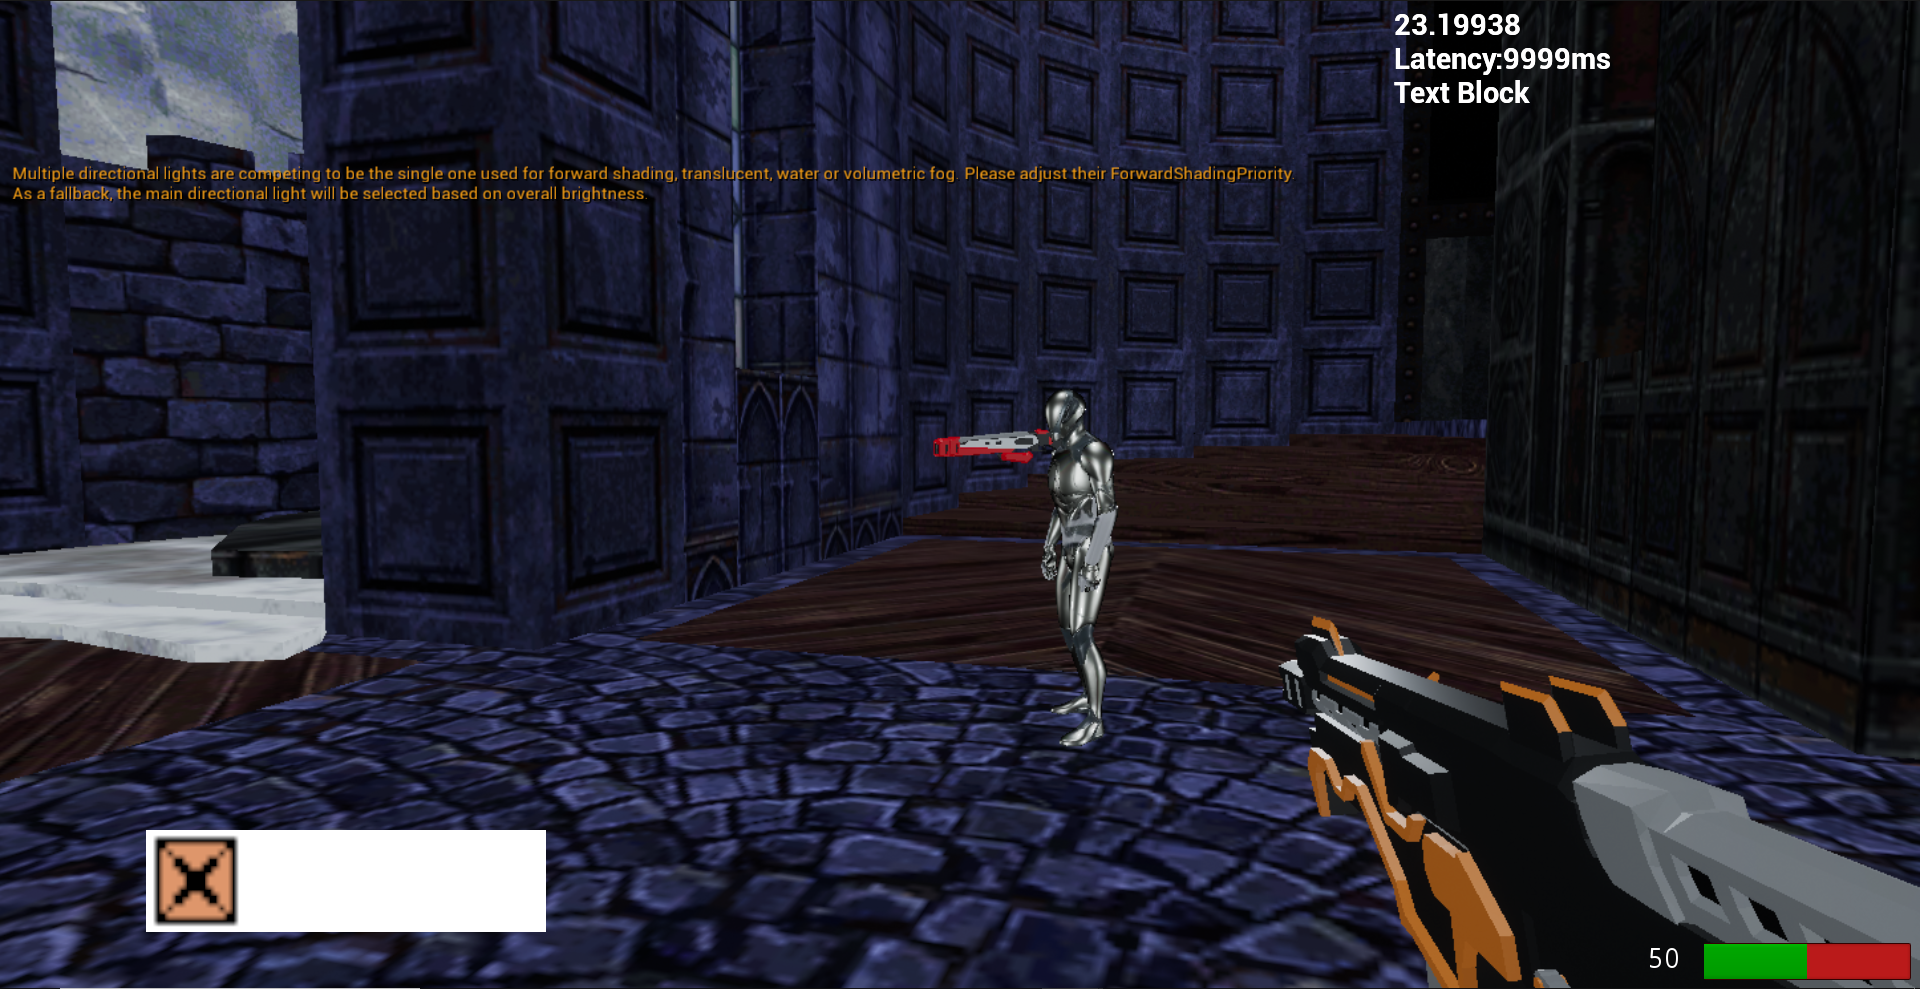
\includegraphics[width=.5\linewidth,right]{figures/NewTest.png}
  \end{figure}
  \bigskip
}

\section{Tools}

\frameT{Map Creation Pipeline} {
	\begin{center}
  		
\includegraphics[width=.8\linewidth]{figures/map_pipeline.png}
  	\end{center}
  	
  	\begin{multicols}{3}
        \begin{itemize}
        		\small
            \item Made in Ultimate Doom Builder
            \item Exported into an .obj file
            \item Import the .obj file into Blender
            \item Export as FBX file
            \item FBX imported into Unreal
            \item Unreal converts to a uasset model
        \end{itemize}
    \end{multicols}
}

\frameT{Test Maps}{
\begin{center}
	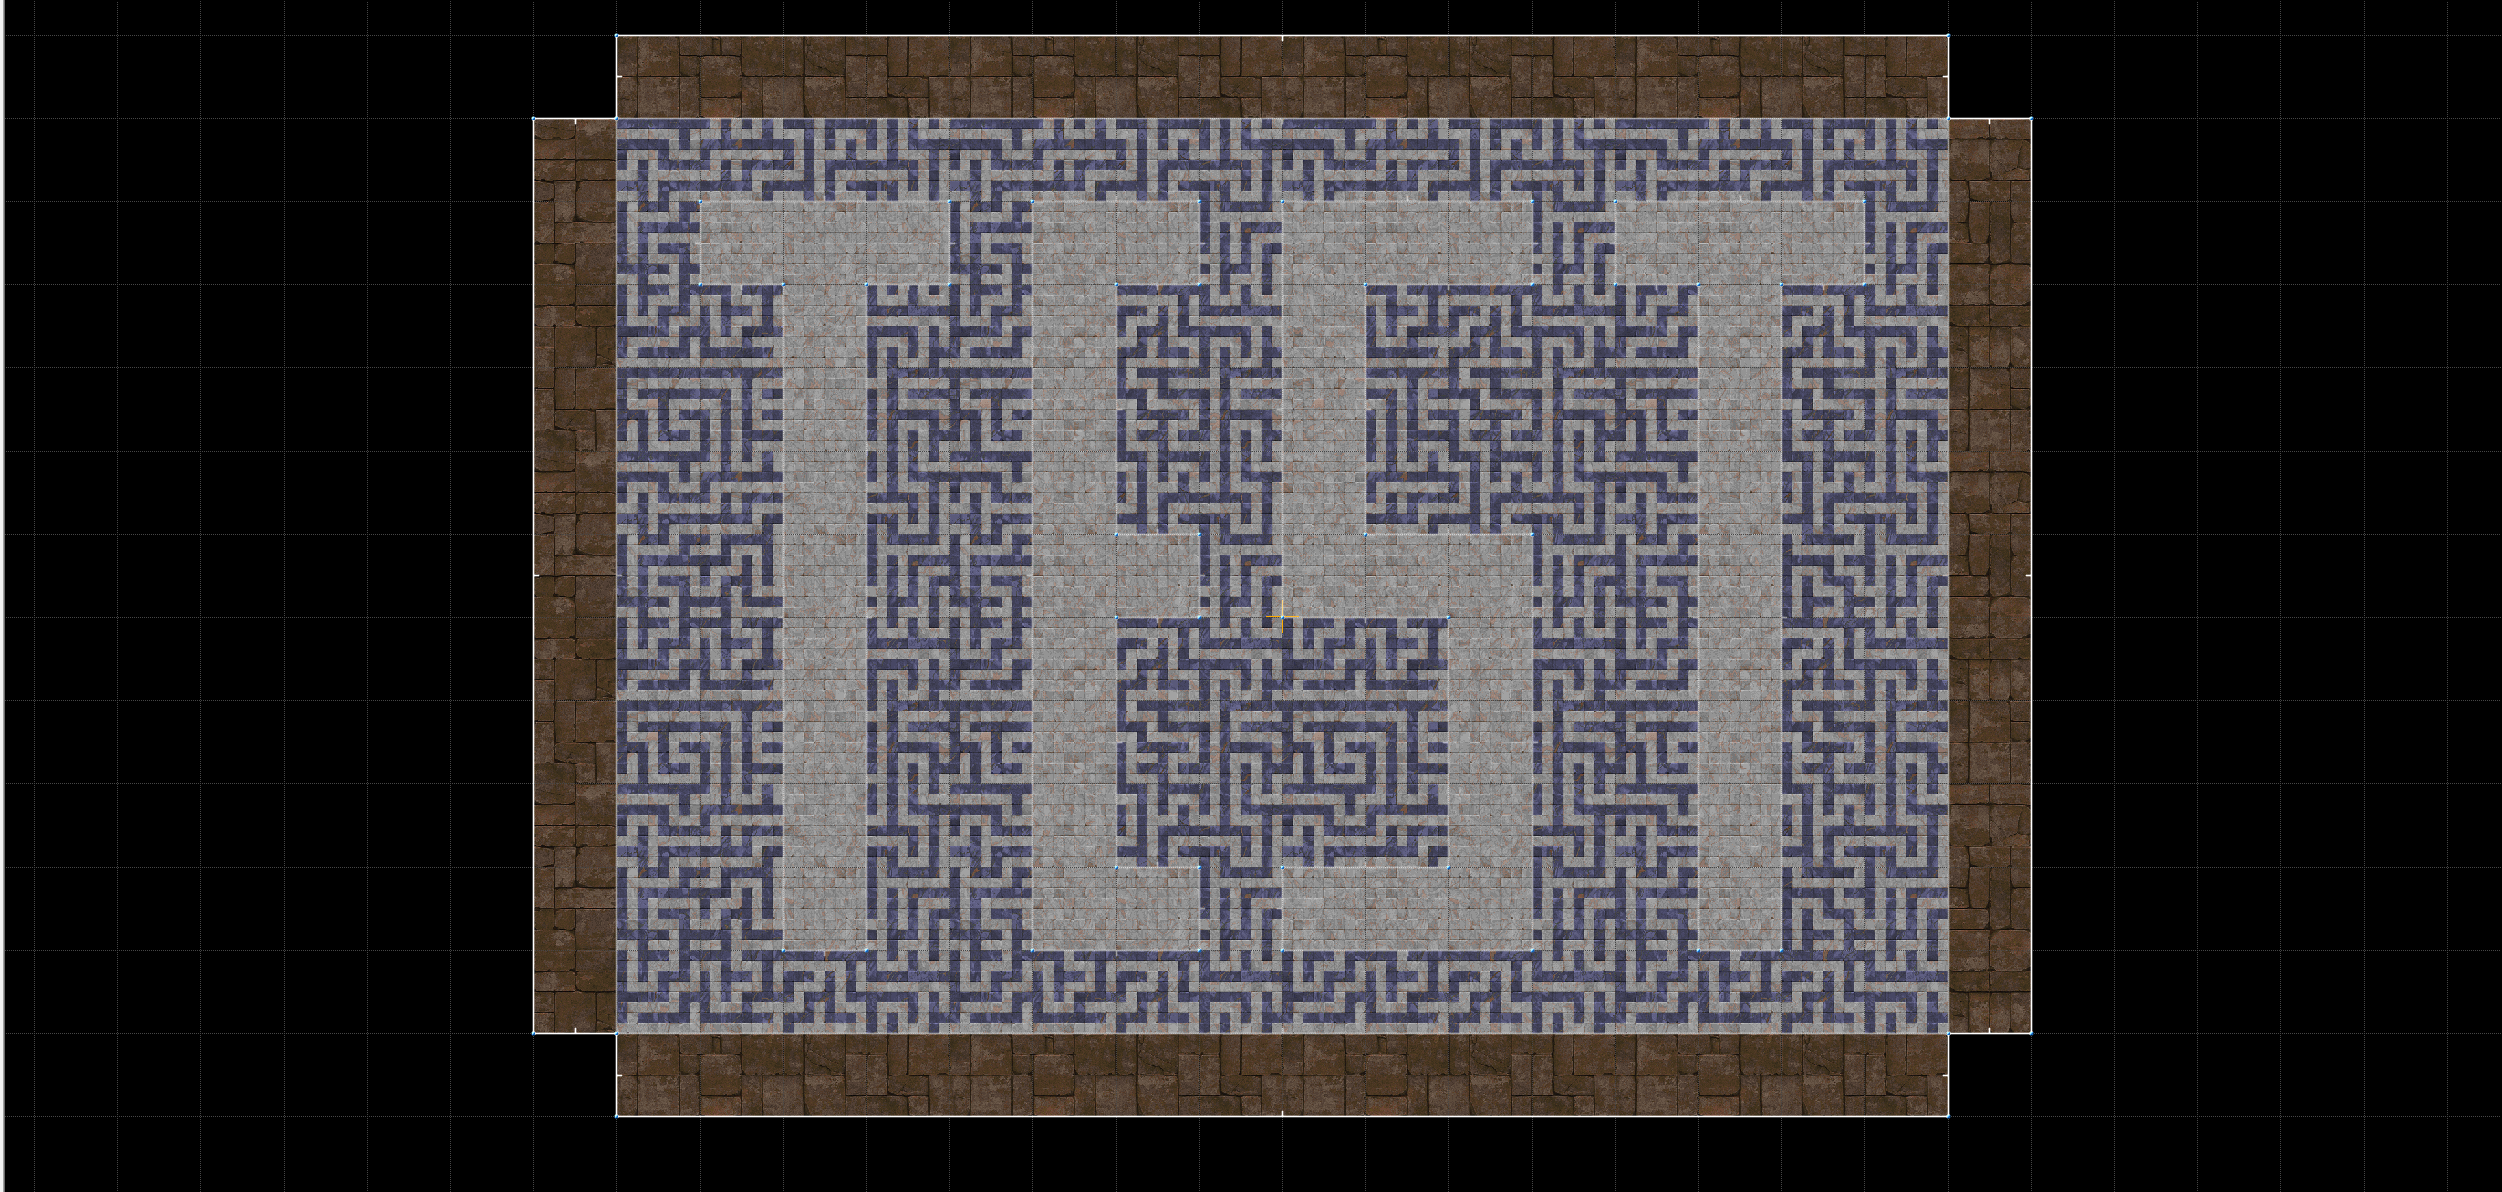
\includegraphics[height=.25\linewidth]{figures/test_map_doom.png}
	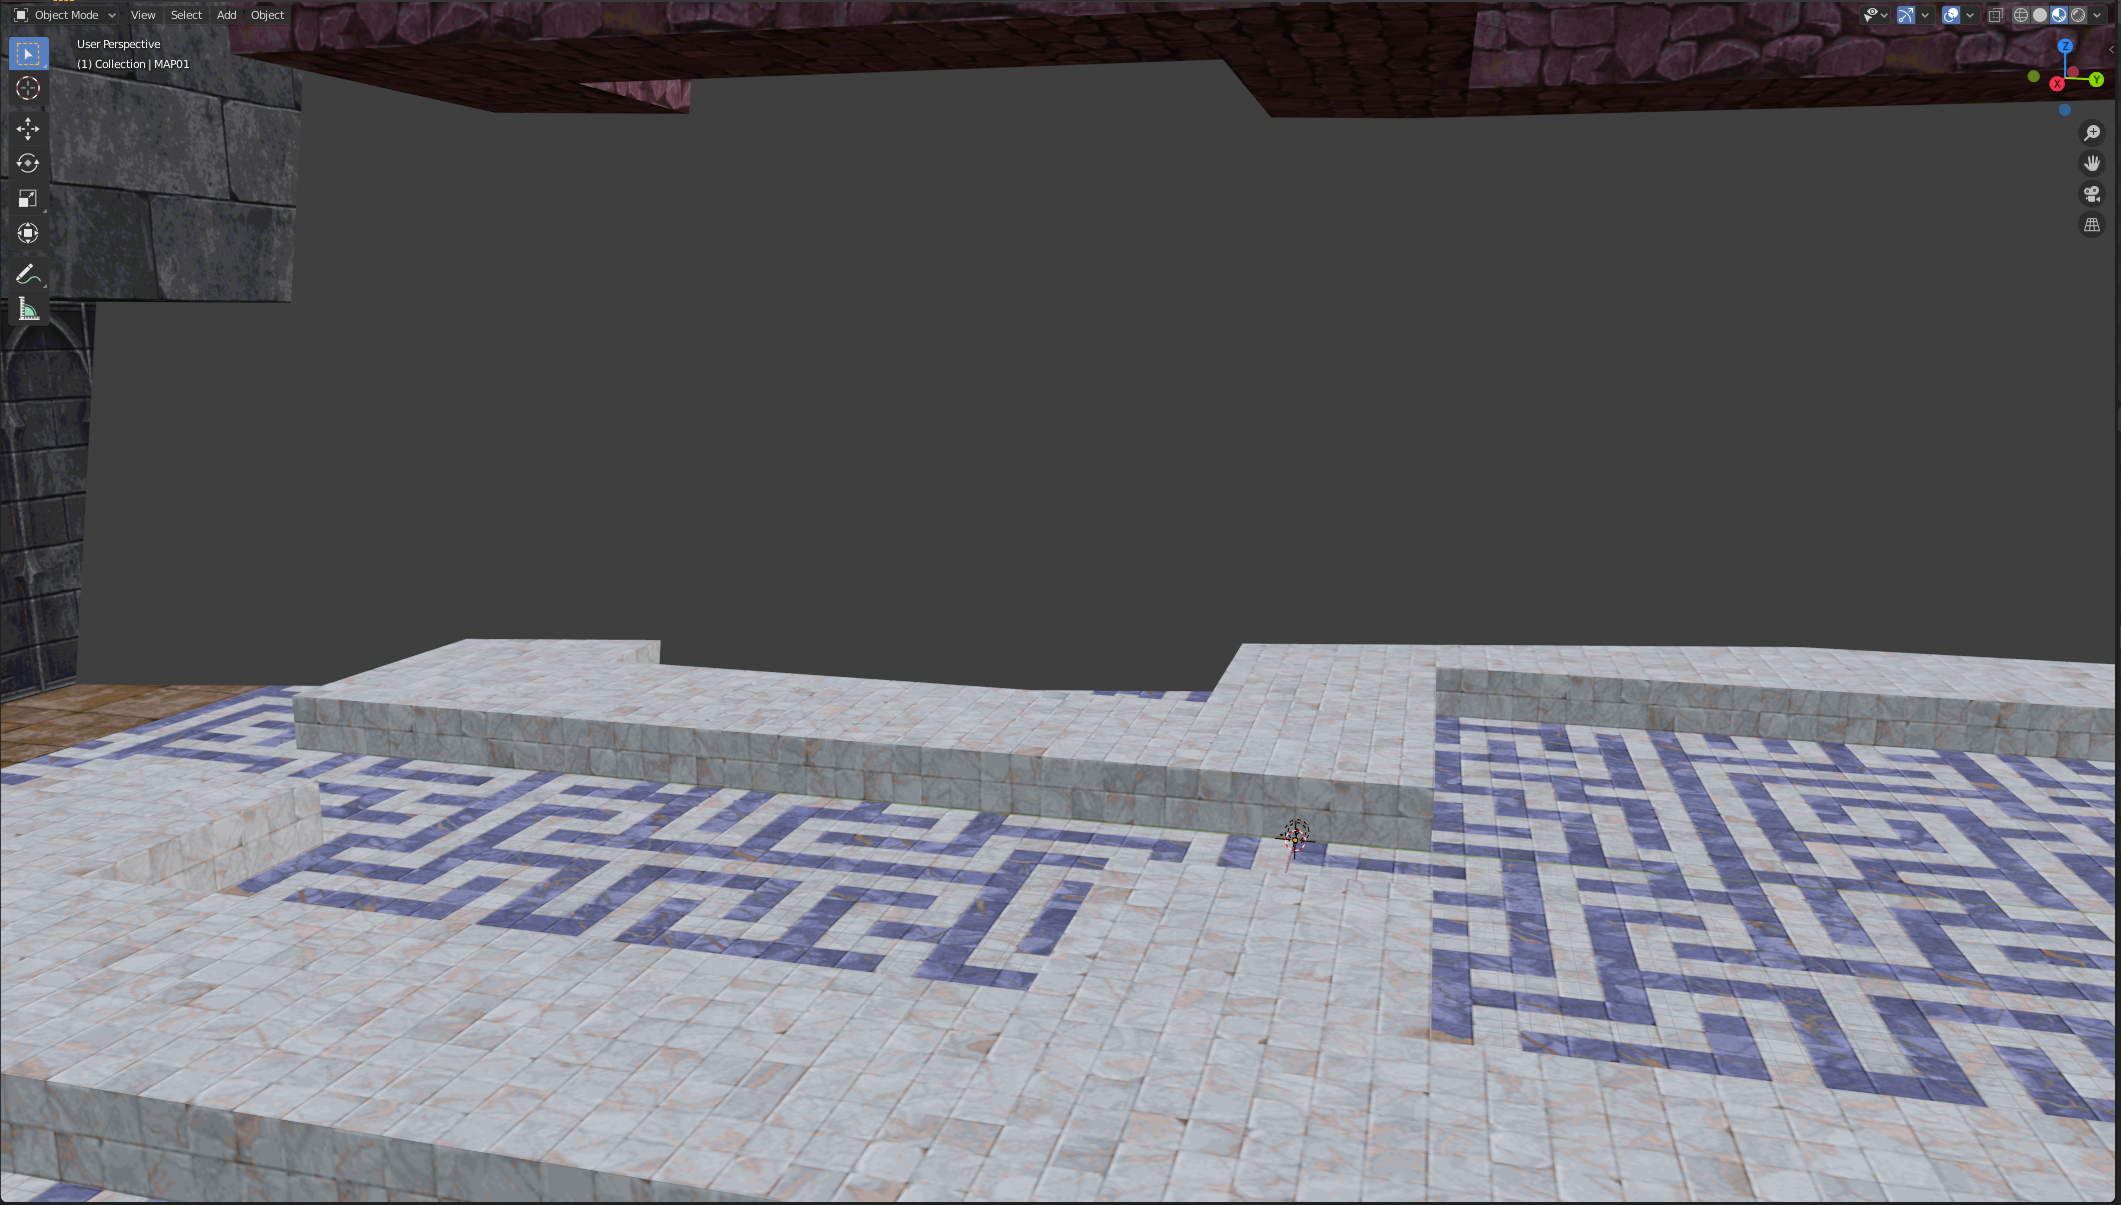
\includegraphics[height=.25\linewidth]{figures/test_map_blender.png}
 \end{center}
 \begin{center}
	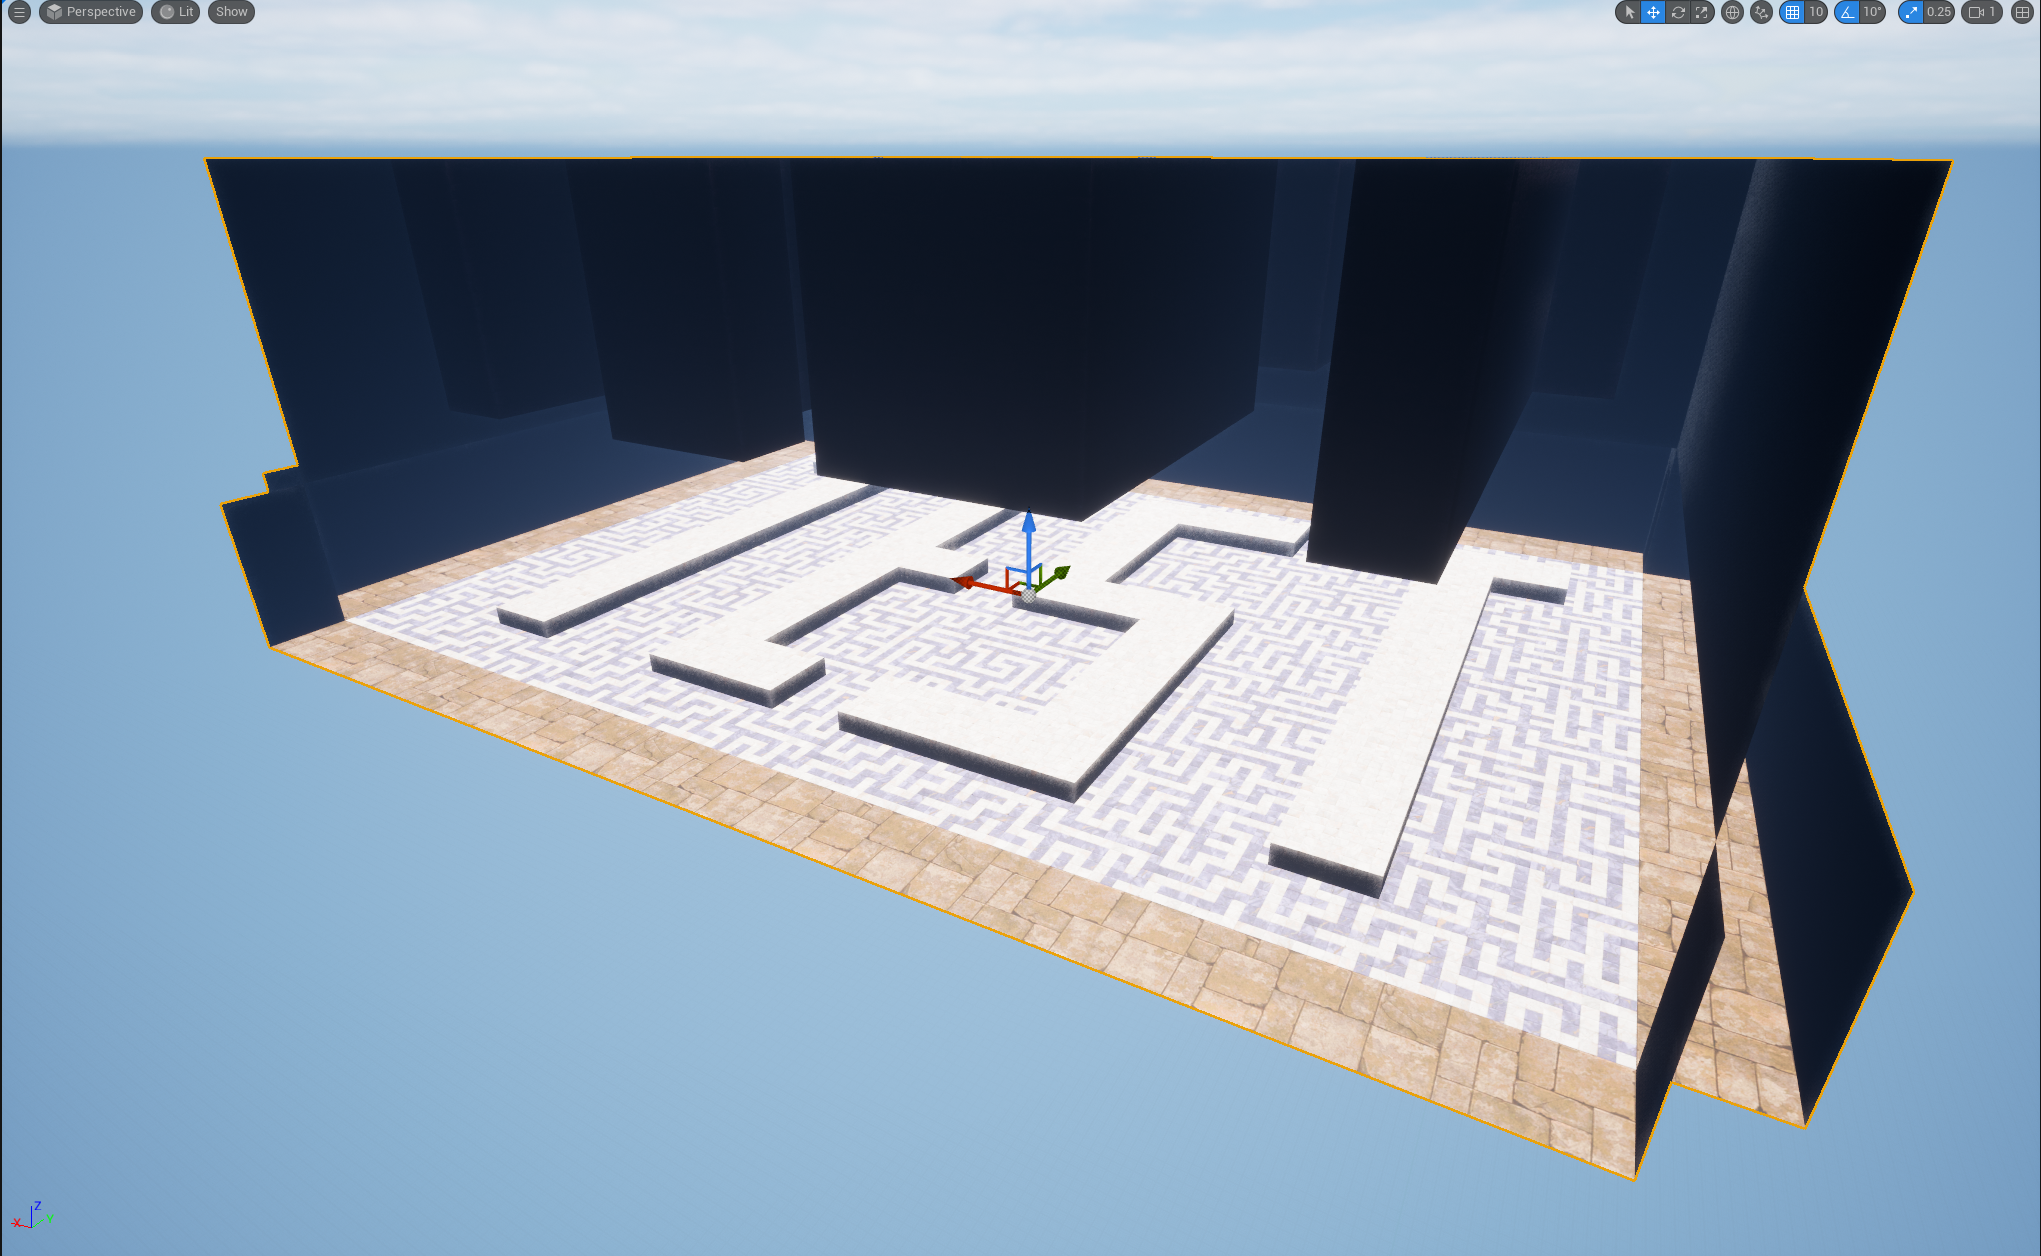
\includegraphics[height=.25\linewidth]{figures/test_map_unreal.png}
 \end{center}
}

\frameT{Networking}{
\begin{center}
	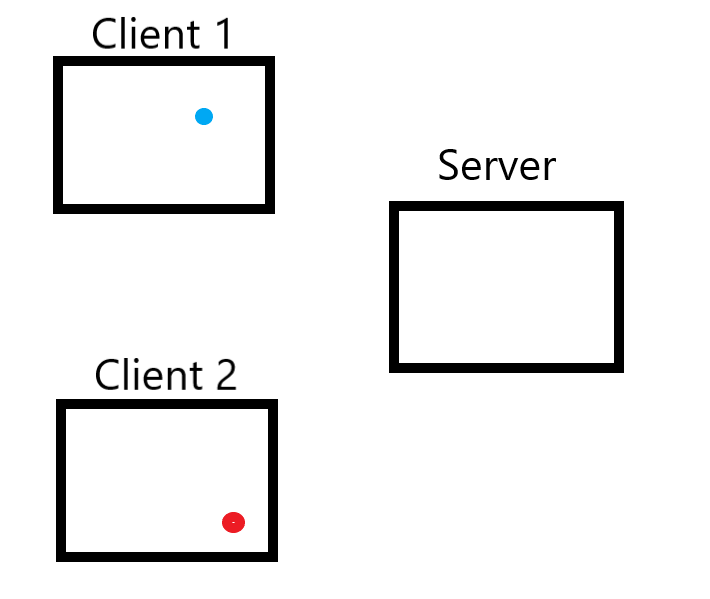
\includegraphics[height=.25\linewidth]{figures/Net1.png}
	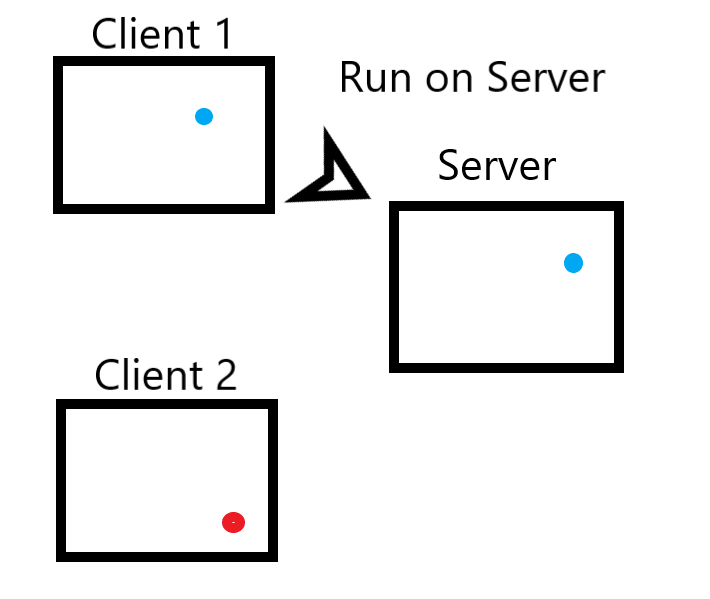
\includegraphics[height=.25\linewidth]{figures/Net2.png}
 \end{center}
 \begin{center}
	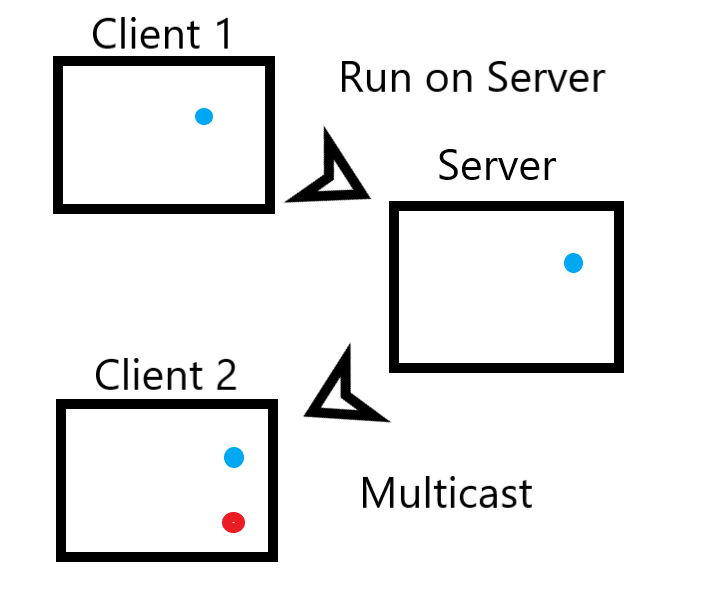
\includegraphics[height=.25\linewidth]{figures/Net3.png}
 \end{center}
}

\frameT{Networking}{
\begin{center}
	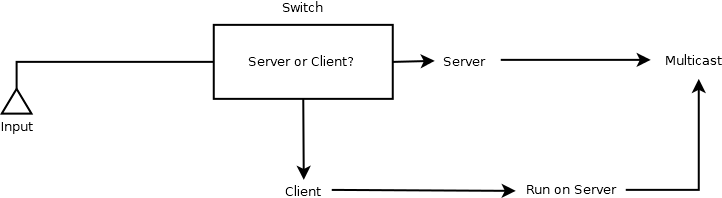
\includegraphics[height=.25\linewidth]{figures/Diagram1.png}
 \end{center}
}

\frameT{Demo}{
%Demo of the player in the game environment.
%	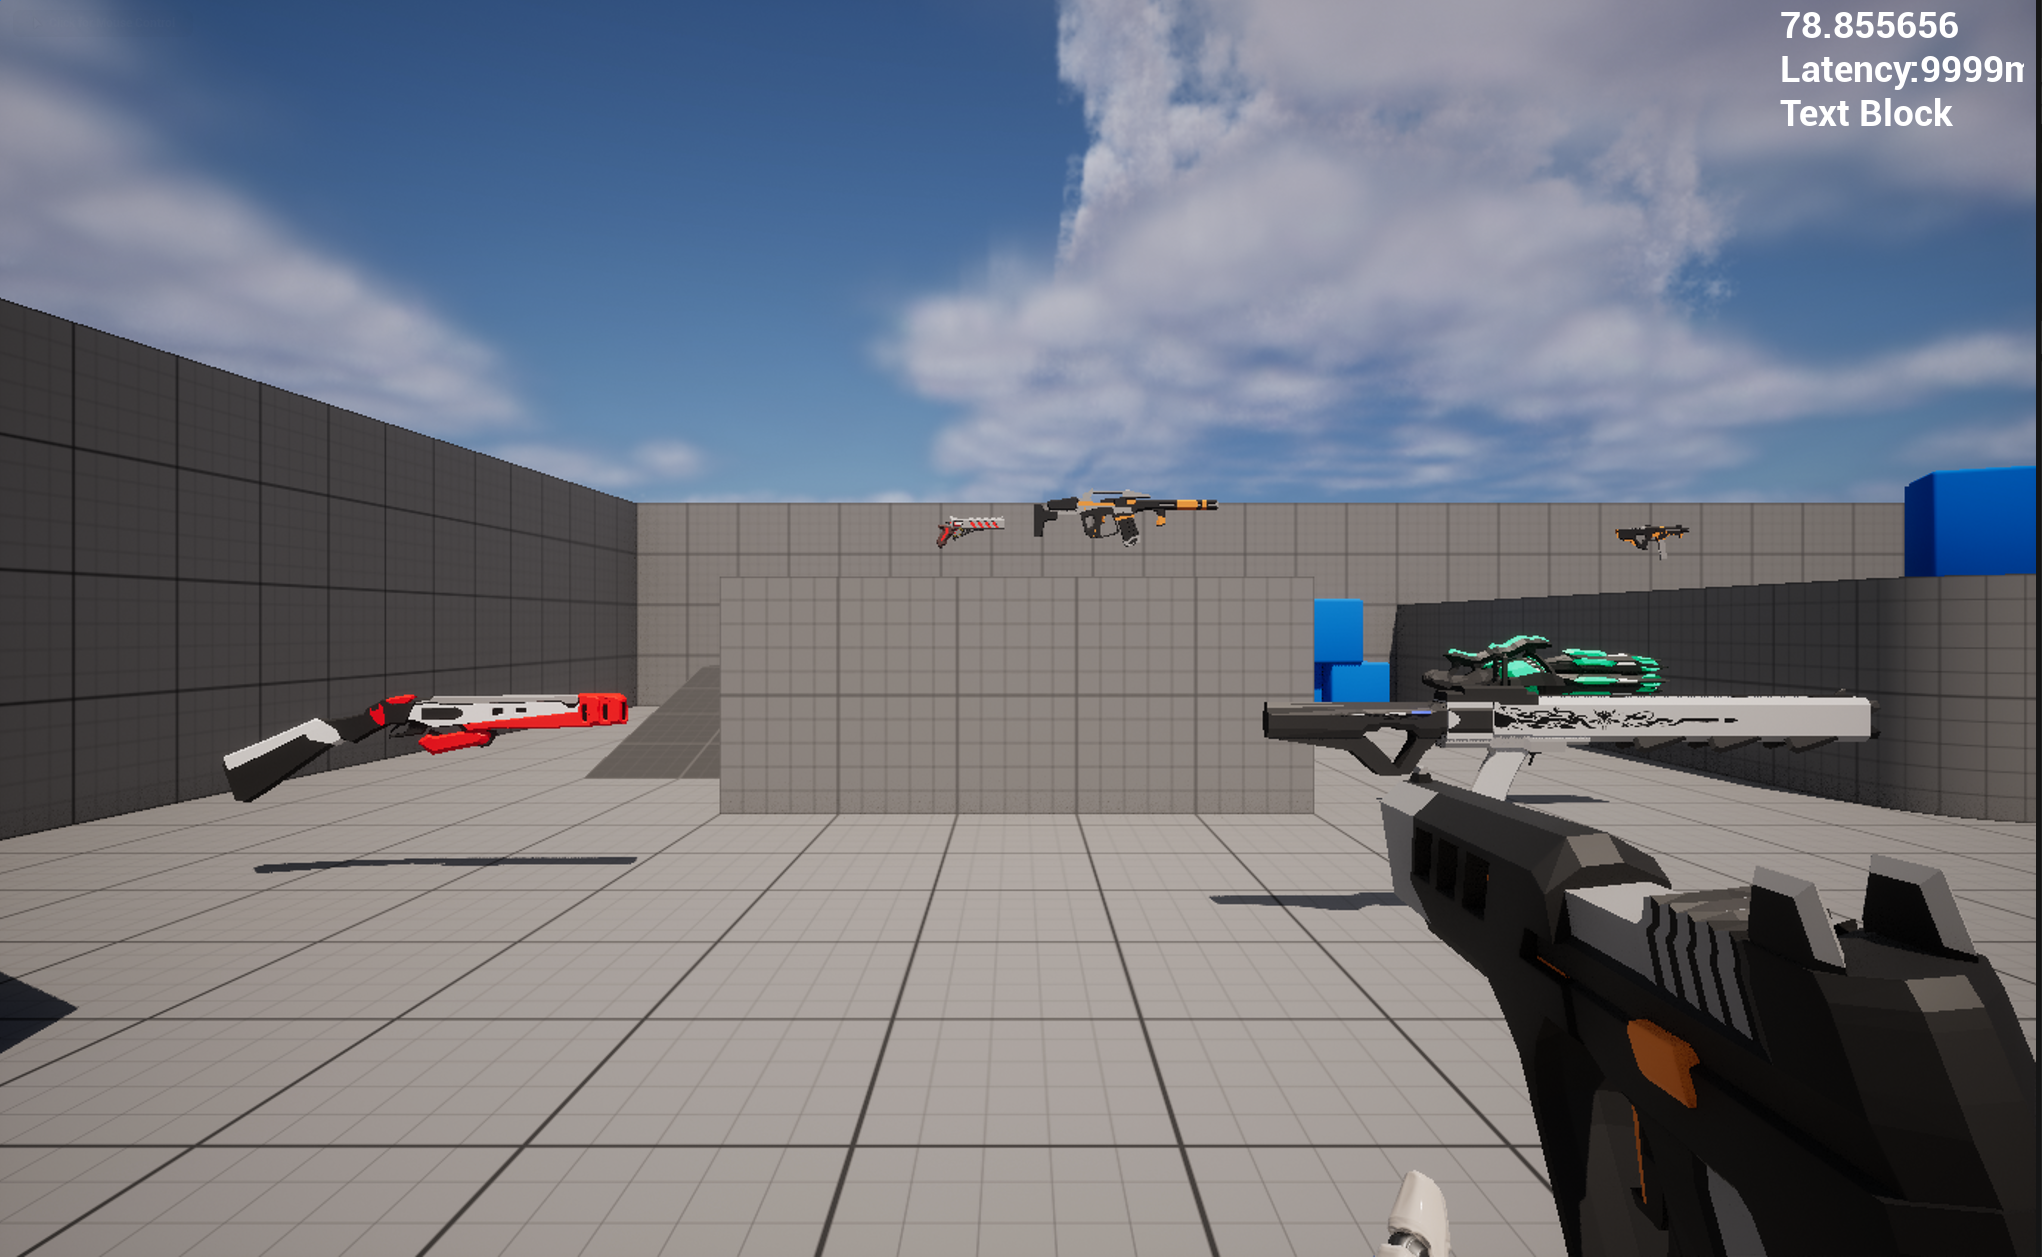
\includegraphics[height=.25\linewidth]{figures/TestDemoGame.png}
}

\frameT{Difficulties}{
  Challenges:
  \bigskip
  \begin{itemize}
      \item Networking
      \item Various weapon related bugs
      \item Hit detection on self
  \end{itemize}
}

\frameT{Future Goals}{
  Goals:
  \bigskip
  \begin{itemize}
      \item Non-local networking
      \item Player scores and win conditions
  \end{itemize}
}
%\Test Online Video!!!!
%\frameT{Demo}{
%\  Demo of the player in the game environment.
  
%\  \bigskip
  
%\  \href{https://www.youtube.com/watch?v=B03EBcuClKs&ab_channel=JaxxonWoods}{Incase of Emergencies}
%\}








%\begin{frame}[fragile]
%\frametitle{Family Tree Knowledge Base}
%Facts:
%\begin{verbatim}
%Verbatim is a great way of enumerating code/algorithmic ideas.
%\end{verbatim}
%\end{frame}
%
%
%\frameT{How to include images} {
%  %% 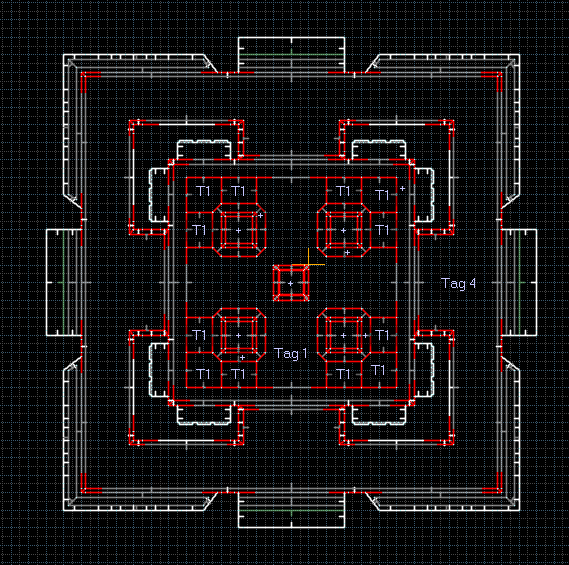
\includegraphics[width=.7\linewidth]{figures/image.pdf}
%}
%
%
%\begin{frame}[fragile]
%  \frametitle{Social Network Graph}
%  \begin{figure}[ht]
%    \begin{minipage}[b]{0.53\linewidth}
%      \centering
%      Minipages are a great way to
%    \end{minipage}
%    \hspace{0.5cm}
%    \begin{minipage}[b]{0.4\linewidth}
%      \centering
%      Line up side-by-side content.
%
%    \end{minipage}
%  \end{figure}
%  
%\end{frame}
%
%
%\frameT{Results} {
%  Describe any results of your work here.
%
%  \bigskip
%
%  Things that worked?
%
%  \bigskip
%
%  Things that didn't work?
%}
%
%\frameT{Conclusions} {
%  Some bullet points here to wrap things up.
%}

\frameT{Any Questions?} {
  
  \begin{center}
    Questions?
  \end{center}
  \begin{center}
    Comments?
  \end{center}

  \bigskip

  Contact Info:
\begin{enumerate}
    \item Victor Gasior: vicagasi@ut.utm.edu
      \bigskip
    \item Blade Johnson: davbjohn@ut.utm.edu
    \bigskip
    \item Andrew Newbill: andjnewb@ut.utm.edu
     \bigskip
    \item Lucky Woods: lucjwood@ut.utm.edu
\end{enumerate}

}

%\frameF{fragile test} {
%}

%% \frameF{Prolog Family Tree} {
%% \begin{verbatim}
%% hello
%% \end{verbatim}



%% }

%Empty Page
%\frameT{Frame 1}{
%}  


\end{document}
